\section{\bt{Evaluation}{实验评估}}
\label{sec:evaluation}
\begin{figure}[t]
\centering
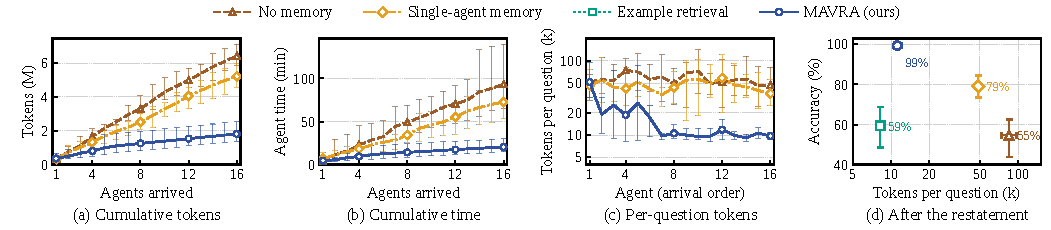
\includegraphics[width=\linewidth]{figures/population}%
\caption{\bt{Sharing across \PpAgents\ sequential agents on TPC-DS before and after a data restatement.}{TPC-DS 上 \PpAgents\ 个顺序到达智能体在数据更正前后的共享效果。}}
\label{fig:population}
\Description{Four panels. Three line charts with capped minimum--maximum error bars compare no memory, single-agent memory, and MAVRA over five runs: cumulative tokens in millions and cumulative agent time in minutes versus the number of agents that have arrived, 1 to 16, and tokens per question of each agent on a log scale. The fourth panel plots accuracy after the restatement against tokens per question on a log scale for the same three methods and example retrieval, with run ranges on both axes.}
\end{figure}

\begin{table}[tb]
\caption{\bt{TPC-DS accuracy and mean cost per question for agents 9--16 (\PpRuns\ runs, tokens include extraction, best values in bold).}{TPC-DS 第 9--16 个智能体的正确率与每题平均代价（\PpRuns\ 轮，token 含提取，最优值加粗）。}}
\label{tab:popcost}
\footnotesize
\setlength{\tabcolsep}{3pt}
\begin{tabularx}{\linewidth}{@{}Lrrrrr@{}}
\toprule
& \bt{LLM}{大模型} & \bt{Tools}{工具} & \bt{Tokens}{token} & \bt{Time}{时间} & \bt{Correct}{正确}\\
\midrule
\bt{No memory}{无记忆} & \PpNoneLateSteps & \PpNoneLateTools & \PpNoneLateTokK\,k & \PpNoneLateS\,s & \PpNoneLateAcc\%\\
\bt{Single-agent memory}{单智能体记忆} & \PpPrivateLateSteps & \PpPrivateLateTools & \PpPrivateLateTokK\,k & \PpPrivateLateS\,s & \PpPrivateLateAcc\%\\
\bt{Example retrieval (shared)}{示例检索（共享）} & \PpTrajLateSteps & \PpTrajLateTools & \textbf{\PpTrajLateTokK\,k} & \PpTrajLateS\,s & \textbf{\PpTrajLateAcc\%}\\
\bt{\textbf{\system\ (ours)}}{\textbf{\system（本文）}} & \textbf{\PpMavraLateSteps} & \textbf{\PpMavraLateTools} & \PpMavraLateTokK\,k & \textbf{\PpMavraLateS\,s} & \PpMavraLateAcc\%\\
\midrule
\bt{\system\ vs.\ no memory}{\system\ 对无记忆} & & & \PpMavraLateTokXNone$\times$ & \PpMavraLateSpeedupNone$\times$ & \\
\bottomrule
\end{tabularx}
\end{table}

\begin{figure*}[t]
\centering
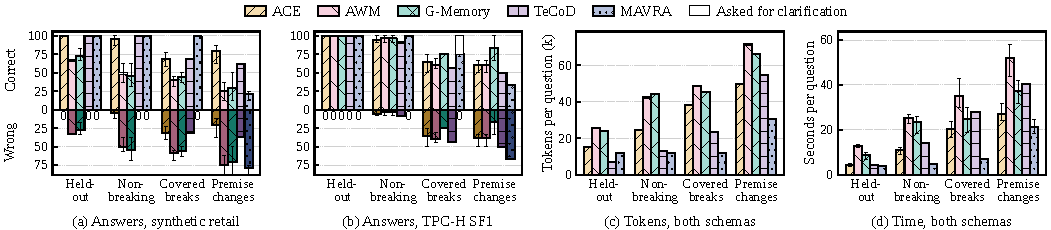
\includegraphics[width=\textwidth]{figures/change-study}%
\caption{\bt{Answer accuracy and per-question cost across 11 data updates on synthetic retail and TPC-H SF1.}{合成零售与 TPC-H SF1 在 11 种数据更新下的作答准确率与单题开销。}}
\label{fig:twoschemas}
\Description{Four grouped bar charts. The first two give, for synthetic retail and TPC-H SF1, the percentage of correct answers (upward bars) and wrong answers (downward bars) of ACE, AWM, G-Memory, TeCoD, and MAVRA on held-out questions, non-breaking updates, breaks covered by conditions, and changes to the domain premises; dashed outlined segments stacked on the correct bars show requests for clarification. The last two give tokens and seconds per scored question for the same groups over both schemas.}
\end{figure*}

\begin{table*}[t]
\caption{\bt{Predictive quality and reuse cost on RelBench.}{RelBench 上的预测质量与复用开销。}}
\label{tab:relbench}
\centering
\small
\setlength{\tabcolsep}{2.8pt}
\renewcommand{\arraystretch}{1.05}
\newcommand{\RbPanelHeader}[4]{%
  \multicolumn{11}{@{}l}{\textbf{#1}}\\[2pt]
  & \multicolumn{6}{c}{\bh{Reuse cost: cutoffs 2--5}{复用代价：截点 2--5}}
  & \multicolumn{3}{c}{\bh{Mean test score: cutoffs 1--5}{平均测试分数：截点 1--5}}
  & \\
  \cmidrule(lr){2-7}\cmidrule(lr){8-10}
  \bh{Method}{方法} & \bh{Tokens\\(M)}{token\\（百万）} & \bh{Token\\ratio}{token\\比率}
  & \bh{LLM\\calls}{LLM\\调用} & \bh{Tool\\calls}{工具\\调用}
  & \bh{Obs.\\min}{观测\\分钟} & \bh{Cost\\(USD)}{美元}
  & #2 & #3 & #4 & \bh{Valid\\sessions}{有效会话}\\
  \midrule
}
\begin{tabular*}{\textwidth}{@{\extracolsep{\fill}}lrrrrrrrrr c@{}}
\toprule
\RbTableBody
\bottomrule
\end{tabular*}
\par\smallskip
\parbox{\textwidth}{\footnotesize\raggedright
\bt{Tokens and dollar costs include memory operations; calls and time cover agent-phase work, excluding leakage audits and background learning. Token ratios are relative to \emph{No memory}. \system{} and \emph{No memory} rows are means over three runs with identical inputs (fractional counts); other methods are single runs. \textsuperscript{*}SQL-adapted FeatPilot (Section~\ref{sec:setup-baselines}).}{token 与费用包含记忆操作；调用次数与时间统计智能体阶段，不包含泄漏审计与后台学习。token 比率以无记忆为基准。\system{} 与无记忆两行为输入相同的三次运行的均值（计数可为小数），其他方法为单次运行。\textsuperscript{*}FeatPilot 的 SQL 适配版本（第~\ref{sec:setup-baselines} 节）。}
}
\end{table*}

\bi{We evaluate \system{} across C1--C3: following the experimental setup (Section~\ref{sec:experimental-setup}), we measure cross-agent definition extraction and sharing on analytical workloads (C1; Section~\ref{sec:population-eval}), natural-language lookup accuracy and latency (C2; Section~\ref{sec:lookup-eval}), validity maintenance and repair under database updates (C3; Section~\ref{sec:changes-eval}), predictive feature reuse on RelBench (C1 and C3; Section~\ref{sec:relbench-eval}), and mechanism ablations with validation overhead (Section~\ref{sec:maint-cost-eval}).}
{我们围绕 C1--C3 系统评估 \system{}：在介绍实验设置（第~\ref{sec:experimental-setup} 节）后，依次评测分析负载上的跨智能体定义提取与共享（C1；第~\ref{sec:population-eval} 节）、自然语言查找的准确性与延迟（C2；第~\ref{sec:lookup-eval} 节）、数据更新下的有效性维护与修复（C3；第~\ref{sec:changes-eval} 节）、RelBench 上的预测特征复用（C1 与 C3；第~\ref{sec:relbench-eval} 节），以及核心机制消融与验证开销（第~\ref{sec:maint-cost-eval} 节）。}

\subsection{\bt{Experimental Setup}{实验设置}}
\label{sec:experimental-setup}
\label{sec:metric-setup}
\bi{\emph{Datasets and workloads.} All experiments run on a 48-vCPU server (Hygon C86 5390, 2.90\,GHz, 98\,GiB RAM, Ubuntu 22.04.5 LTS, PostgreSQL 18.6). The TPC-DS SF1~\cite{tpcds2026benchmark} population study spans 24 tables (2.9M \code{store\_sales} rows) and five metrics, each paired with two learning questions and five evaluation forms (new periods, period differences, and monthly rankings). The eleven-update study evaluates three metrics per schema on synthetic retail (1M sales, 396k returns, 500k catalog sales) and TPC-H SF1~\cite{tpch2026benchmark}, while fixed-library replay additionally covers SSB~\cite{oneil2009ssb} and BIRD \code{financial}~\cite{li2023bird}. For predictive modeling, RelBench~\cite{robinson2024relbench} provides six classification and regression tasks on \code{rel-stack} and \code{rel-trial} across five temporal cutoffs spaced 91 and 365 days apart (210 sessions total; cutoff~5 matches the official split).}
{\emph{数据集与工作负载。}全部实验运行于 48 逻辑 CPU 服务器（Hygon C86 5390，2.90\,GHz，98\,GiB 内存，Ubuntu 22.04.5 LTS，PostgreSQL 18.6）。TPC-DS SF1~\cite{tpcds2026benchmark} 群体实验涵盖 24 张表（\code{store\_sales} 含 290 万行）与五个指标，每个指标设两道学习题及五种评测题型（新期间、跨期差值与月度排名）。十一类更新实验在合成零售库（100 万行销售、39.6 万行退货、50 万行目录销售）与 TPC-H SF1~\cite{tpch2026benchmark} 上各评测三个指标；固定定义库回放进一步覆盖 SSB~\cite{oneil2009ssb} 与 BIRD \code{financial}~\cite{li2023bird}。预测建模采用 RelBench~\cite{robinson2024relbench} 在 \code{rel-stack} 与 \code{rel-trial} 上的六项分类与回归任务，跨五个间隔 91 天与 365 天的时间截点评测（共 210 个会话，第五截点对应官方划分）。}

\label{sec:setup-baselines}
\label{sec:setup-metrics}
\bi{\emph{Baselines, models, and metrics.} For analytical sharing, \emph{Single-agent memory} runs \system{}'s extraction and maintenance privately per agent, \emph{No memory} retains state within a single question, and \emph{Example retrieval} shares verified question--SQL pairs without maintenance. Across analytical updates and predictive tasks, we compare SQL-adapted ACE~\cite{zhang2026ace} (80k-token private playbook maintained by Reflector/Curator prompts), AWM~\cite{wang2025awm} (online SQL workflow induction), G-Memory~\cite{zhang2025gmemory} (shared hierarchical memory), TeCoD~\cite{jivani2025tecod} (shared NLI-matched SQL templates with three examples), and---for predictive tasks---FeatPilot*~\cite{liang2025featpilot} (join-path search ranked by coverage times LightGBM importance). Agents use \code{deepseek-flash} (\llmmodel{}, 20-turn cap, 60--120\,s SQL timeout, $\le 3$ lookups/question; predictive sessions budget 40 planner calls and 8 LightGBM 4.6.0~\cite{ke2017lightgbm} validations on 50k rows). Reported tokens include all memory operations; in update studies, clarification requests and execution errors receive no credit and mismatched values count as wrong.}
{\emph{基线、模型与评价指标。}分析共享实验中，\emph{单智能体记忆}在各智能体内部私有运行与 \system{} 相同的提取与维护逻辑，\emph{无记忆}仅保留单题上下文，\emph{示例检索}跨智能体共享核验问题与 SQL 但不做维护。在分析更新与预测任务上，我们对比 SQL 适配版 ACE~\cite{zhang2026ace}（由 Reflector／Curator 维护的 80k-token 私有手册）、AWM~\cite{wang2025awm}（在线 SQL 工作流归纳）、G-Memory~\cite{zhang2025gmemory}（共享层次化记忆）、TeCoD~\cite{jivani2025tecod}（基于蕴含匹配的共享 SQL 模板及三条示例），以及面向预测任务的 FeatPilot*~\cite{liang2025featpilot}（按覆盖率乘以 LightGBM 重要性排序的连接路径搜索）。智能体统一采用 \code{deepseek-flash}（\llmmodel{}，20 轮上限，60--120\,s SQL 超时，每题至多三次查找；预测会话预算为 40 次规划调用与 8 次 5 万行 LightGBM 4.6.0~\cite{ke2017lightgbm} 验证）。总 token 计入所有记忆读写开销；更新实验中请求澄清与执行报错不计正确，数值不符计为错答。}

\subsection{\bt{Cross-Agent Sharing on Analytical Queries}{分析查询上的跨智能体共享}}
\label{sec:overall-eval}
\label{sec:population-eval}
\label{sec:sharing-eval}
\bi{We first evaluate whether definitions extracted from early sessions (C1) amortize exploration cost across a sequential agent population, holding extraction and maintenance fixed via \emph{Single-agent memory}. Across five paired runs starting from empty memory, \PpAgents{} agents arrive sequentially and each answers seven of 35 TPC-DS questions in matched order (2,240 sessions). Without memory, cumulative tokens grow linearly with agent arrivals (Figure~\ref{fig:population}a--c), while \emph{Single-agent memory} reuses definitions only when the same agent revisits a metric. \system{} publishes \PpMavraLearns{} definitions per run from verified sessions and reuses them on \PpMavraReused\% of questions, consuming \PpMavraTotalTokM\,M total tokens (\PpMavraTokSaveNone\% below \emph{No memory} and \PpMavraTokSavePrivate\% below \emph{Single-agent memory}) while raising accuracy to \PpMavraAcc\% (vs.\ \PpNoneAcc\% and \PpPrivateAcc\%). Once the catalog warms up (agents 9--16), \system{} averages 10.0\,k tokens per question at \PpMavraLateAcc\% accuracy, delivering a \PpMavraLateSpeedupNone$\times$ latency speedup over \emph{No memory} (Table~\ref{tab:popcost}).}
{我们首先检验早期会话提取的定义（C1）能否在顺序到达的智能体群体间摊销探查成本，并以提取和维护机制完全相同的\emph{单智能体记忆}作为对照。五轮从空记忆启动的配对运行中，\PpAgents{} 个智能体依次到达，按匹配顺序从 35 道 TPC-DS 题中各答 7 题（共 2,240 个会话）。无记忆下累计 token 随智能体到达呈线性增长（图~\ref{fig:population}a--c），单智能体记忆仅能在同一智能体再次遇到相同指标时复用。\system{} 每轮从核验会话发布 \PpMavraLearns{} 个定义并在 \PpMavraReused\% 的问题上实现复用，总消耗仅 \PpMavraTotalTokM\,M token（较无记忆与单智能体记忆分别节省 \PpMavraTokSaveNone\% 与 \PpMavraTokSavePrivate\%），同时将整体准确率提升至 \PpMavraAcc\%（对照分别为 \PpNoneAcc\% 与 \PpPrivateAcc\%）。目录预热后（第 9--16 个智能体），\system{} 每题平均仅耗 10.0\,k token，准确率达 \PpMavraLateAcc\%，平均单题延迟较无记忆加速 \PpMavraLateSpeedupNone{} 倍（表~\ref{tab:popcost}）。}

\subsection{\bt{Lookup Accuracy}{查找准确性}}
\label{sec:lookup-eval}
% Lookup study (Section V-C). Sources: exp/2026-11-10-lookup-facets/
%   results-baselines/summary.json (name match, embedding, LLM methods; LLM methods two runs each),
%   results-ft/ft/base-dc-xl-s1{3,4,5}/summary.json (single judge, 82/83/85 of 96),
%   results-ft/serve-ens3/serve-summary.json (three judges end to end: first ask and repeated wording),
%   results-ft/recall-latency.json (bge-m3 recall, 17 ms).
% Unified metrics (review point 4, 2026-11-11): first-response set-exact, final set-exact after the consuming agent's
% confirmation turn (exp/2026-11-11-maint-hardening/lookup-confirm: deepseek-flash reads MAVRA's references and picks),
% absent requests rejected, LLM tokens (prompt + completion) and seconds per request including confirmation.
\begin{table}[htbp]
\caption{\bt{Lookup on 96 requests over 26 TPC-DS definitions, in one metric for all methods.}{26 条 TPC-DS 定义上 96 个请求的查找结果（所有方法统一口径）。}}
\label{tab:lookup}
\footnotesize
\setlength{\tabcolsep}{3.0pt}
\begin{tabularx}{\columnwidth}{@{}L r r r r r@{}}
\toprule
\textbf{\bt{Method}{方法}} & \textbf{\bt{Exact}{一致}} & \textbf{\bt{Final}{确认后}} & \textbf{\bt{Absent}{拒识}} & \textbf{\bt{LLM tok.}{LLM token}} & \textbf{\bt{Time}{耗时}}\\
\midrule
\bt{Exact name match}{精确名称匹配} & 42\% & 42\% & 14/17 & 0 & --\\
\bt{Embedding top-1 (oracle thr.)}{向量 top-1（最优阈值）} & 62\% & 62\% & 6/17 & 0 & 17\,ms\\
\bt{Full-catalog LLM judge}{全目录 LLM 判别} & 99\% & 99\% & 17/17 & 1{,}534 & 2.2\,s\\
\bt{Top-8 recall + LLM judge}{Top-8 召回 + LLM 判别} & 98\% & 98\% & 16/17 & 760 & 2.0\,s\\
\bt{LLM choice parser + Def.~\ref{def:consistency}}{LLM 口径解析 + 定义~\ref{def:consistency}} & 90\% & 90\% & 16/17 & 971 & 5.2\,s\\
\bt{TeCoD template matcher (NLI)}{TeCoD 模板匹配（NLI）} & 26\% & 26\% & 17/17 & 0 & 60\,s$^{*}$\\
\midrule
\bt{Single cross-encoder judge}{单交叉编码器判别器} & 85--89\% & -- & -- & 0 & 33\,ms\\
\textbf{\system{}}, \bt{first-time phrasing}{首次表述} & 92\% & \textbf{99\%} & 17/17 & 89 & 0.53\,s\\
\textbf{\system{}}, \bt{repeated phrasing}{同表述再查} & 98\% & -- & 13/13 & 0 & 33\,ms\\
\bottomrule
\end{tabularx}
\par\smallskip
{\raggedright
\bt{Exact: the first response (direct answer, or the references returned) equals $A(\rho)$. Final: after the consuming agent (\llmmodel{}) picks among \system{}'s references on the 23\% of requests that receive them. Absent: out-of-catalog requests finally rejected (per run). Tokens and time are means per request, confirmation included (shared GPU for judges; API for LLMs). $^{*}$Released 4B embedding and NLI models in float32 on a shared CPU; pool of 6 phrasings per definition from the same catalog-generated data.}{一致：首次响应（直接答案，或返回的参考集合）等于 $A(\rho)$。确认后：对收到参考的 23\% 请求，由使用方智能体（\llmmodel{}）在参考中选择之后的结果。拒识：目录外请求最终被拒识的数量（每轮）。token 与耗时为每请求均值，含确认（判别器运行于共享 GPU，LLM 经 API 调用）。$^{*}$TeCoD 发布的 4B 嵌入与 NLI 模型以 float32 运行于共享 CPU；模板池为每个定义 6 条取自同一份目录生成数据的问法。}\par}
\end{table}

\bi{Because questions in Sections~\ref{sec:population-eval} and~\ref{sec:changes-eval} state canonical metric names, we evaluate lookup independently on a stress-test catalog of 26 TPC-DS definitions containing three homonymous pairs (store revenue after vs.\ before coupons, store returns attributed by return vs.\ sale date, and store return rate by amount vs.\ units) alongside dense near-neighbors across profit/margin, coupon/discount, unit/revenue, and channel/category variants. Prior to running any method, we authored 96 benchmark requests spanning six categories: canonical names (23), paraphrases (27), explicit choice specifications (18), underspecified terms such as ``store profit'' (4), near-miss distractors (7), and out-of-catalog metrics (17). Ground-truth target sets $A(\rho)$ (Definition~\ref{def:consistency}) contain one definition on 61 requests, two on 18, and none on 17. Judges are trained exclusively on catalog-synthesized phrasings with thresholds fixed a priori at $0.1$ and $0.9$ (no test-set tuning) on a shared NVIDIA RTX 5880 Ada GPU; LLM baselines call \code{deepseek-flash}.}
{由于第~\ref{sec:population-eval} 与~\ref{sec:changes-eval} 节的问题显式给出了标准指标名，我们构建了包含 26 条 TPC-DS 定义的压力测试目录对查找模块进行专项评估：其中包括三对同名异义定义（扣券后与扣券前的门店营业额、按退货日与销售日归属的门店退货额、按金额与件数计算的门店退货率）以及在利润／毛利、优惠券／折扣、销量／销售额、渠道／品类上高度邻近的变体。在运行任何方法前，我们预先手工编写了涵盖六类情形的 96 个测试请求：标准名称（23）、同义改写（27）、显式口径说明（18）、``门店利润''等欠明确表述（4）、字面相近干扰项（7）以及目录外指标（17）。按定义~\ref{def:consistency} 确定的真值集合 $A(\rho)$ 中，61 题对应唯一定义，18 题对应两条定义，17 题为空集。判别器仅在目录自动合成的表述上训练，阈值预先固定为 $0.1$ 与 $0.9$（未在测试集调参），运行于单块共享 NVIDIA RTX 5880 Ada GPU；LLM 基线调用 \code{deepseek-flash}。}

\bi{Table~\ref{tab:lookup} summarizes the accuracy--latency trade-off. Exact name matching fails on all paraphrases (42\% exact). Even under an oracle threshold, top-1 embedding similarity resolves 0 of 18 two-definition requests and misclassifies 11 of 17 absent requests as hits. Prompting an LLM with the full catalog achieves 99\% exact match, but incurs 2.2\,s latency and 1.3k prompt tokens per lookup that scale with catalog size, whereas LLM choice parsing reaches 90\% at 5.2\,s. A single cross-encoder judge resolves 82--85 of 96 requests (85--89\%) in 33\,ms. Combining the three-seed ensemble with confidence thresholding, \system{} answers 77\% of first-time requests directly at 98.6\% precision and returns references containing $A(\rho)$ on the remainder---yielding 99\% usable resolution in 0.18\,s without LLM calls. Re-queried with new time parameters, 79 requests hit the alias table and 96\% resolve directly at 100\% precision.}
{表~\ref{tab:lookup} 展示了准确率与延迟的权衡。精确名称匹配无法处理任何同义改写（完全一致率仅 42\%）。向量相似度即便采用事后最优阈值，在 18 个双定义请求上完全一致率仍为 0，且将 17 个目录外请求中的 11 个误判为命中。让 LLM 审阅全目录虽可达到 99\% 完全一致率，但每次查找需 2.2\,s 与随目录膨胀的 1.3k 输入 token；改用 LLM 解析口径则降至 90\%（耗时 5.2\,s）。单个交叉编码器在 33\,ms 内可完全答对 96 题中的 82--85 题（85--89\%）。结合三种子集成与置信度分级决策后，\system{} 在不调用 LLM 的前提下以 0.18\,s 延迟直接回答 77\% 的首次查询（准确率 98.6\%），其余请求返回的参考均覆盖 $A(\rho)$，整体可用率达 99\%。更换时间参数再次查询时，79 个请求直接命中别名表，96\% 实现 100\% 准确率的直接响应。}

\bi{\emph{Training scale and zero-shot new definitions.} Single-seed exact matches rise monotonically with synthetic phrasing volume (51, 77, 84, and 85 of 96 at 347, 693, 3,466, and 6,933 phrasings; full-data seeds span 82--85), dropping to 82 when structural differences are omitted from candidate inputs and to 81 without out-of-catalog intents. Crucially, when five definitions (including a homonymous pair) are held out from training entirely, requests targeting them still achieve 11/13 exact matches (85\%) across all three seeds---matching the 82\% rate on seen definitions and confirming that newly published definitions are resolved without retraining. Cross-candidate attention via a set layer or Set-Encoder listwise head matched independent scoring (85/96 each).}
{\emph{合成数据规模与新定义零样本泛化。}单种子完全一致数随合成表述数量单调上升（347、693、3,466 与 6,933 条表述下分别为 96 题中的 51、77、84 与 85 题；全量数据跨种子为 82--85 题）；若移除候选输入中的结构差异描述则降至 82 题，移除目录外合成意图则降至 81 题。关键在于，将 5 条定义（含一对同名定义）从训练阶段完全留出后，针对这些未见定义的请求在三个种子上均取得 11/13（85\%）的完全一致率，与已见定义（82\%）持平，证实新发布的定义无需重训判别器即可被准确检出。引入跨候选注意力的集合层或 Set-Encoder 列表判别头与独立打分表现一致（均为 85/96）。}

\subsection{\bt{Reuse Under Data Updates}{数据更新下的有效性维护与修复}}
\label{sec:changes-eval}
\label{sec:scenarios}
\label{sec:validity}
\bi{\emph{Maintaining shared knowledge.} Following the 16-agent TPC-DS run, we apply a restatement update that supersedes historical sales rows, and each returning agent answers four affected questions (320 sessions per method). \system{} detects the grain-uniqueness break, repairs the shared definitions once, and answers \PpMavraChangeAcc\% correctly at \PpMavraChangeTokK\,k tokens per question; \emph{Example retrieval} spends comparable tokens, but its unmaintained SQL aggregates superseded rows and drops to \PpTrajChangeAcc\% accuracy (Figure~\ref{fig:population}d).}
{\emph{共享知识的维护。}在 16 智能体 TPC-DS 实验结束后，我们施加替代历史销售记录的数据重述更新，每个智能体返回回答四道受影响问题（每方法 320 个会话）。\system{} 检出粒度唯一性违例并对共享定义执行一次性修复，以每题 \PpMavraChangeTokK\,k token 答对 \PpMavraChangeAcc\%；\emph{示例检索}的 token 开销相近，但未经维护的历史 SQL 误读被替代行，准确率骤降至 \PpTrajChangeAcc\%（图~\ref{fig:population}d）。}

\bi{\emph{Comparison with agent memories.} We next evaluate eleven independent updates on synthetic retail and TPC-H SF1 across \CsRuns{} runs (Figure~\ref{fig:twoschemas}), comprising four \emph{non-breaking updates}, five \emph{condition-breaking updates} (status rows, versioned corrections, and duplicate loads breaking key uniqueness; dimension history breaking join cardinality; date re-keying breaking date joins), and two \emph{domain-premise shifts} (unit change B2; backup copy B1). After learning each metric from two formula-bearing questions, agents answer single-month and period-difference questions by metric name (\CsQuestions{} scored questions per run). Across both schemas, \system{} answers \CsBreakMavra\% of condition-breaking questions correctly with \emph{zero} wrong answers---automatically repairing unambiguous breaks and withholding definitions on a TPC-H late batch lacking ship dates, where every baseline answers all \CsTpchLatekeyN{} questions wrong; overall on breaking updates, baselines achieve only \CsBreakBaseMin--\CsBreakBaseMax\% accuracy with \CsBreakBaseWrongMin--\CsBreakBaseWrongMax\% wrong answers (Figure~\ref{fig:twoschemas}a,b). Moreover, \system{} achieves 100\% accuracy on held-out and non-breaking questions at the lowest overall cost (\CsAllMavraTokK\,k tokens and \CsAllMavraS\,s vs.\ \CsAllBaseTokMinK--\CsAllBaseTokMaxK\,k tokens and \CsAllBaseSMin--\CsAllBaseSMax\,s for baselines; \CsBreakMavraS\,s vs.\ \CsBreakBaseSMin--\CsBreakBaseSMax\,s on breaking updates).}
{\emph{与智能体记忆方法的对比。}我们在合成零售库与 TPC-H SF1 上跨 \CsRuns{} 轮独立评测十一类更新（图~\ref{fig:twoschemas}），涵盖四类\emph{常规更新}、五类\emph{条件破坏更新}（状态流水、版本更正与重复装载破坏键唯一性，维表历史破坏连接基数，日期重编码破坏日期连接）以及两类\emph{领域前提变更}（单位变更 B2、备份副本 B1）。智能体先从两道含公式题学习各指标，再仅凭指标名回答单月及跨期差值问题（每轮 \CsQuestions{} 道计分题）。跨两种模式，\system{} 在条件破坏题上取得 \CsBreakMavra\% 准确率并保持\emph{零错答}——自动修复无歧义违例，并在缺失发货日期的 TPC-H 批次上停用定义（所有基线在该批次全部 \CsTpchLatekeyN{} 题上均答错）；整体而言，基线在条件破坏题上的准确率仅为 \CsBreakBaseMin--\CsBreakBaseMax\%，错答率高达 \CsBreakBaseWrongMin--\CsBreakBaseWrongMax\%（图~\ref{fig:twoschemas}a,b）。同时，\system{} 答对 100\% 的留出题与常规更新题，并取得最低总体开销（每题 \CsAllMavraTokK\,k token、\CsAllMavraS\,s，基线为 \CsAllBaseTokMinK--\CsAllBaseTokMaxK\,k token、\CsAllBaseSMin--\CsAllBaseSMax\,s；条件破坏题上为 \CsBreakMavraS\,s 对 \CsBreakBaseSMin--\CsBreakBaseSMax\,s）。}

\bi{\emph{Domain-premise shifts and probe-lifted assumptions.} Under the backup-copy update (B1), filtering on either source tag restores key uniqueness, so data alone cannot identify the authoritative source; \system{} detects the non-unique repair and withholds the definition rather than guessing, answering \CsMirrorMavraC{} of \CsMirrorN{} questions correctly (tied with TeCoD for highest), whereas silent unit changes (B2) require an updated business specification.}
{\emph{领域前提变更与探查提取假设。}在备份副本更新（B1）下，按任一来源标签过滤均可恢复键唯一性，仅凭数据无法判定权威来源；\system{} 检出修复候选非唯一后停用定义而非盲目猜测，答对 \CsMirrorN{} 题中的 \CsMirrorMavraC{} 题（与 TeCoD 并列最高），而无数据痕迹的单位变更（B2）则需更新业务说明。}

\subsection{\bt{Predictive Feature Reuse}{预测特征复用}}
\label{sec:relbench-eval}
\begin{figure}[t]
\centering
% Vector drawing generated by tools/figures/relbench_cumulative.py from exp/2026-10-20-relbench/paper-sessions.json; rerun it after the numbers change.
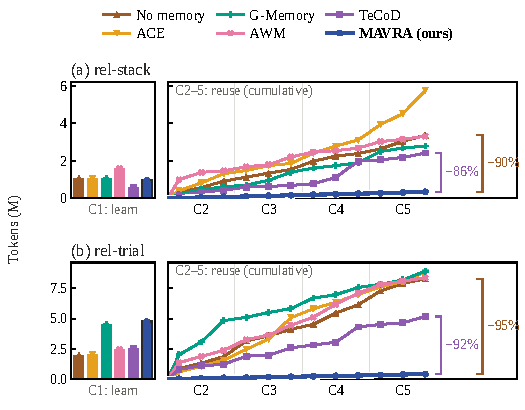
\includegraphics[width=\linewidth]{figures/relbench-cumulative}%
\caption{\bt{Tokens with memory operations: learning at cutoff 1 (bars) and cumulative reuse over cutoffs 2--5 (lines). Brackets give \system{}'s reuse-stage saving.}{含记忆操作的 token：截点 1 的学习（柱）与截点 2--5 的累计复用（折线）。括号标出 \system{} 复用阶段的节省。}}
\label{fig:relbench-cumulative}
\Description{Two rows, rel-stack and rel-trial, share one legend. In each row, a narrow bar chart on the left shows the tokens each of six LLM-based methods spent in the three learning sessions of cutoff 1, and a line chart on the right, on the same token axis, shows cumulative tokens over the twelve reuse sessions of cutoffs 2 to 5, starting from zero. MAVRA's line ends lowest in both rows; brackets mark its saving relative to TeCoD, the cheapest baseline, and to No memory.}
\end{figure}

\ifbilingual\begin{figure}[tb]\else\begin{figure}[t]\fi
\centering
\ifbilingual
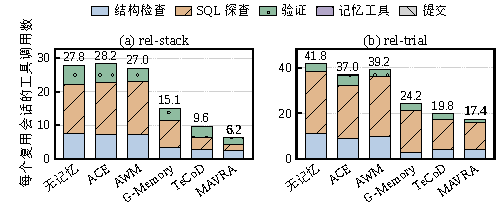
\includegraphics[width=\linewidth]{figures/reuse-work-zh}
\else
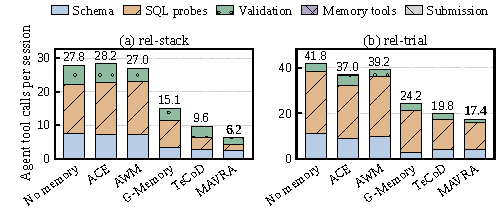
\includegraphics[width=\linewidth]{figures/reuse-work}
\fi
\caption{\bt{Agent-issued tool calls per reuse session at cutoffs 2--3 (six sessions per method and database, failures included).}{截点 2--3 每个复用会话的智能体工具调用数（每种方法、每个数据库六个会话，含失败）。}}
\label{fig:reuse-work}
\Description{Two side-by-side panels, one per database, compare all five methods. Stacked bars distinguish schema inspection, SQL probes, validation, memory tools, and submission with colors and hatching. The y-axis counts agent-issued tool calls per reuse session and starts at zero.}
\end{figure}

\bi{Across the five-cutoff RelBench study, \system{} achieves the lowest reuse-stage tokens, LLM calls, tool calls, wall-clock time, and monetary cost among all methods on both databases (Table~\ref{tab:relbench}). Relative to \emph{No memory}, reuse-stage tokens drop by \RbStackMavraTokSave\% on \code{rel-stack} and \RbTrialMavraTokSave\% on \code{rel-trial}; including initial cutoff-1 learning and all memory operations, end-to-end tokens still fall by \RbStackMavraTokSaveAll\% and \RbTrialMavraTokSaveAll\% (Figure~\ref{fig:relbench-cumulative}). \system{} completes all 15 sessions per database with valid, leak-free pipelines (whereas \emph{No memory}, ACE, and AWM suffer invalid or temporally leaking runs), attains the best user-engagement AUC (\RbStackMavraQC{}), and improves test quality over \emph{No memory} on post-votes, user-engagement, and site-success. Against the lowest-cost baseline TeCoD, \system{} cuts reuse tokens by a further \RbStackMavraVsBest\% and \RbTrialMavraVsBest\% by replacing repetitive probing with compiled task programs and feature definitions: per reuse session, \system{} issues only \RbStackMavraExplore{} and \RbTrialMavraExplore{} schema/SQL probes versus \RbStackNoneExplore{} and \RbTrialNoneExplore{} without memory (Figure~\ref{fig:reuse-work}).}
{在五截点 RelBench 预测评测中，\system{} 在两个数据库复用阶段的 token 用量、LLM 调用数、工具调用数、耗时与费用均为所有方法最低（表~\ref{tab:relbench}）。相比无记忆，\code{rel-stack} 与 \code{rel-trial} 复用阶段 token 分别下降 \RbStackMavraTokSave\% 与 \RbTrialMavraTokSave\%；计入首截点学习及全部记忆操作后，端到端总 token 仍减少 \RbStackMavraTokSaveAll\% 与 \RbTrialMavraTokSaveAll\%（图~\ref{fig:relbench-cumulative}）。\system{} 在每库全部 15 个会话中均产出合法且无时间泄漏的方案（无记忆、ACE 与 AWM 均出现无效或时间泄漏会话），取得最优 user-engagement AUC（\RbStackMavraQC{}），并在 post-votes、user-engagement 与 site-success 上优于无记忆基线。相比开销最低的基线 TeCoD，\system{} 凭借已核验任务程序与编译特征替代重复探查，进一步节省 \RbStackMavraVsBest\% 与 \RbTrialMavraVsBest\% 的复用 token：每个复用会话仅发起 \RbStackMavraExplore{} 与 \RbTrialMavraExplore{} 次模式／SQL 探查，而无记忆高达 \RbStackNoneExplore{} 与 \RbTrialNoneExplore{} 次（图~\ref{fig:reuse-work}）。}

\subsection{\bt{Mechanism Analysis and Overhead}{机制消融与系统开销}}
\label{sec:maint-cost-eval}
\begin{table}[htbp]
\caption{\bt{Maintenance policy replay across \RpTotal\ instances, four schemas, twelve update classes (correct / wrong / withheld). Premise changes: unit, backup copy, reclassification.}{维护策略在四种模式、十二类更新共 \RpTotal\ 个实例上的回放结果（正确 / 错误 / 拒答）。前提变更：单位、备份副本、维度改类。}}
\label{tab:replay-policies}
\footnotesize
\setlength{\tabcolsep}{2.5pt}
\begin{tabularx}{\linewidth}{@{}Lccc@{}}
\toprule
& \bt{Non-breaking}{常规更新} & \bt{Covered breaks}{条件破坏} & \bt{Premise changes}{前提变更}\\
\bt{Maintenance policy}{维护方式} & (\RpBenignN) & (\RpBreakN) & (\RpOutsideN)\\
\midrule
\bt{Invalidate on every write}{每次写入即失效} & \RpRevokeBenignC\,/\,\RpRevokeBenignW\,/\,\RpRevokeBenignR & \RpRevokeBreakC\,/\,\RpRevokeBreakW\,/\,\RpRevokeBreakR & \RpRevokeOutsideC\,/\,\RpRevokeOutsideW\,/\,\RpRevokeOutsideR\\
\bt{Schema check only}{只检查模式} & \RpSchemaBenignC\,/\,\RpSchemaBenignW\,/\,\RpSchemaBenignR & \RpSchemaBreakC\,/\,\RpSchemaBreakW\,/\,\RpSchemaBreakR & \RpSchemaOutsideC\,/\,\RpSchemaOutsideW\,/\,\RpSchemaOutsideR\\
\bt{dbt-style table tests}{dbt 式表级测试} & \RpTestsBenignC\,/\,\RpTestsBenignW\,/\,\RpTestsBenignR & \RpTestsBreakC\,/\,\RpTestsBreakW\,/\,\RpTestsBreakR & \RpTestsOutsideC\,/\,\RpTestsOutsideW\,/\,\RpTestsOutsideR\\
\bt{\textbf{\system\ (ours)}}{\textbf{\system（本文）}} & \textbf{\RpMavraBenignC}\,/\,\RpMavraBenignW\,/\,\RpMavraBenignR & \textbf{\RpMavraBreakC}\,/\,\RpMavraBreakW\,/\,\RpMavraBreakR & \RpMavraOutsideC\,/\,\RpMavraOutsideW\,/\,\RpMavraOutsideR\\
\bottomrule
\end{tabularx}
\end{table}

\begin{figure}[tb]
\centering
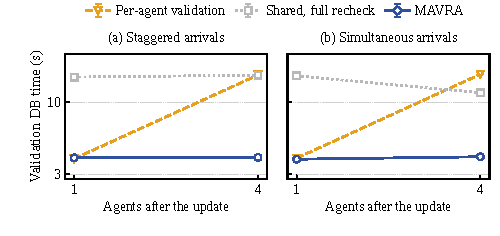
\includegraphics[width=\linewidth]{figures/shared-validation}%
\caption{\bt{Validation database time after an incremental load as 1--\SvAgentsMax\ agents query 16 shared definitions.}{增量装载后 1--\SvAgentsMax\ 个智能体查询 16 个共享定义时的验证数据库耗时。}}
\label{fig:fixed-sharing}
\Description{Two log-log line charts, staggered and simultaneous arrivals, plot validation database time in seconds against the number of agents, 1 to 32. Per-agent validation rises in proportion to the number of agents; shared full recheck stays flat at a higher level; MAVRA stays flat at the lowest level. Error bars span three randomized blocks.}
\end{figure}

\bi{\emph{Publication gates and maintenance policies.} Across \PubAllJudged{} verified sessions, compiled-answer replay (G7) and arithmetic-trace checks (G2) intercept \PubReplayRefused{} lossy extractions whose compiled SQL misses the verified answer and \PubChainRefused{} candidates with inconsistent traces prior to publication. Replaying \RpTotal{} question instances against fixed catalogs across four schemas (Table~\ref{tab:replay-policies}), \emph{Invalidate on every write} discards all definitions; \emph{Schema check only} serves silent wrong answers on \RpSchemaBreakWPct\% of condition-breaking instances; and \emph{dbt-style table tests}~\cite{dbt2026tests} disable every definition touching a failing table. \system{} serves exact answers on all non-breaking updates and on \RpMavraBreakC{} of \RpBreakN{} condition-breaking instances (\RpMavraBreakCPct\%), with only \RpMavraBreakW{} wrong outputs and \RpMavraBreakR{} withheld.}
{\emph{发布门禁与维护策略消融。}在 \PubAllJudged{} 个核验会话中，编译答案复现（G7）与算术推导链核查（G2）分别在发布前拦截了 \PubReplayRefused{} 个编译 SQL 偏离核验答案的有损提取，以及 \PubChainRefused{} 个算术链不一致的候选。表~\ref{tab:replay-policies} 在四种数据库模式上对固定目录回放 \RpTotal{} 个题次：\emph{每次写入即失效}丢弃全部定义；\emph{只检查模式}在 \RpSchemaBreakWPct\% 的条件破坏题次上静默返回错答；\emph{dbt 式表级测试}~\cite{dbt2026tests}则停用受影响表上的全部定义。\system{} 在全部常规更新及 \RpBreakN{} 个条件破坏题次中的 \RpMavraBreakC{} 个（\RpMavraBreakCPct\%）上返回正确结果，仅出现 \RpMavraBreakW{} 个错答与 \RpMavraBreakR{} 个停用。}

\bi{\emph{Two-stage filtering and shared validation.} Publishing 16 definitions across four fact/date table pairs (200k rows per fact table) and appending new keys as 1--\SvAgentsMax{} agents query all definitions (Figure~\ref{fig:fixed-sharing}), \system{} executes a constant \SvStagMavraChecks{} condition checks regardless of agent concurrency, whereas \emph{Per-agent validation} and \emph{Shared full recheck} incur \SvStagPrivateRatio$\times$ and \SvStagFullRatio$\times$ as much validation database time at \SvAgentsMax{} staggered agents (\SvSimPrivateRatio$\times$ and \SvSimFullRatio$\times$ under simultaneous arrivals).}
{\emph{两级筛选与共享验证开销。}在四对事实／日期表（每张事实表 20 万行）上发布 16 个定义并追加新键，随 1--\SvAgentsMax{} 个智能体并发查询全部定义（图~\ref{fig:fixed-sharing}），\system{} 无论智能体规模如何均仅执行恒定的 \SvStagMavraChecks{} 次条件检查；在 \SvAgentsMax{} 个智能体错峰到达时，逐智能体独立验证与共享全量重查耗费的数据库验证时间分别为 \system{} 的 \SvStagPrivateRatio{} 倍与 \SvStagFullRatio{} 倍（同时到达下分别为 \SvSimPrivateRatio{} 倍与 \SvSimFullRatio{} 倍）。}

\bi{\emph{Shared repair.} Following the TPC-DS restatement, repairing each shared definition once consumes \PpMavraMaintS\,s of total database time versus \PpPrivateMaintS\,s across private agent copies, amortizing the repair cost in $M(\pi)$ across the population.}
{\emph{共享修复开销。}TPC-DS 数据重述后，对共享定义执行单次统一修复仅耗费 \PpMavraMaintS\,s 数据库时间，而各智能体分别维护私有副本共需 \PpPrivateMaintS\,s，有效在群体间摊销了维护代价 $M(\pi)$ 中的修复项。}
